\section{Tecnologías}
Para el desarrollo del proyecto se propone utilizar las siguientes tecnologías que permitirán lograr los objetivos propuestos en el sistema. Las ventajas que representan para el desarrollo son descritas a continuación.
\vspace{-15mm}
	\begin{table}[b!]
    \centering
      \begin{tabular}{|p{2cm}|ll}
        \hline
        \multicolumn{2}{|c|}{{\bf Cuadro comparativo de tecnologías}} \\ 
        \hline
          \multicolumn{1}{|p{4cm}|}{{\bf Nombre}} & 
		  \multicolumn{1}{p{10cm}|}{{\bf Características}}\\

        \hline
          \multicolumn{1}{|p{5cm}|}{
\includegraphics[width=0.3\textwidth]{images/neo4j}} & 
          \multicolumn{2}{p{10cm}|}{\begin{itemize}
          \vspace{-15mm}
        \item Es una base de datos open-source,esta escrita en java.
        \item Permite realizar transacciones ACID.
        \item Manera su propio lenguaje de query , Cypher.
        \item Puede contener billiones de nodos y relaciones.
        \item Rápido recorriendo relaciones, este tipo de queries se conoce como transversals
        \item Las escrituras se pueden realizar en cualquier instancia del clúster.
        \item Multilenguaje, proporciona una Api Rest pudiendo utilizarse desde cualquier lenguaje.
      \end{itemize}} \\
         
        \hline
          \multicolumn{1}{|p{5cm}|}{
\includegraphics[width=0.3\textwidth]{images/InfiniteGraph}} & 
          \multicolumn{1}{p{10cm}|}{
          \begin{itemize}
          \vspace{-7mm}
        \item Posee almacenamiento en la nube.
        \item Apoyo de consultas en paralelo.
        \item Precios felixibles y opciones de licencia.
        \item Totalmente transaccional y multi-hilo,
      \end{itemize}} \\ 
        \hline
          \multicolumn{1}{|p{3cm}|}{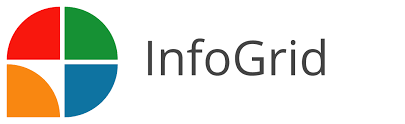
\includegraphics[width=0.3\textwidth]{images/InfoGrid}} & 
          \multicolumn{1}{p{10cm}|}{
          \begin{itemize}
          \vspace{-10mm}
        \item Recorrido Gráfico y consultas de tipo relacional.
        \item Indexación personalizable.
        \item Gestión de almacenamiento personalizable.
      \end{itemize}}\\ 
         \hline
        %\hline
      \end{tabular}
      \caption{Bases de datos Orientadas a Grafos}
      \label{Analisis de riesgos}
    \end{table}
\newpage
\begin{table}[b!]
    \centering
      \begin{tabular}{|p{1cm}|l}
        \hline
        \multicolumn{2}{|c|}{{\bf Cuadro comparativo de tecnologías}} \\ 
        \hline
          \multicolumn{1}{|p{4cm}|}{{\bf Nombre}} & 
		  \multicolumn{1}{p{10cm}|}{{\bf Características}}\\
		 \hline
          \multicolumn{1}{|p{5cm}|}{
\includegraphics[width=0.3\textwidth]{images/bootstrap}} & 
          \multicolumn{1}{p{10cm}|}{\begin{itemize} 
       \vspace{-20mm}
          \item Es un framework o conjunto de herramientas de software libre para diseño de sitios y aplicaciones web. 
        \item Contiene plantillas de diseño con tipografía, formularios, botones, cuadros, menús de navegación y otros elementos de diseño basado en HTML y CSS, así como, extensiones de JavaScript opcionales adicionales.
        \item Es compatible con la mayoría de los navegadores web.
        \item Bootstrap es de código abierto y está disponible en GitHub. 
        \item Desde la versión 2.0 también soporta diseños sensibles. Esto significa que el diseño gráfico de la página se ajusta dinámicamente, tomando en cuenta las características del dispositivo usado (Computadoras, tabletas, teléfonos móviles).
      \end{itemize}} \\
         
        \hline
          \multicolumn{1}{|p{5cm}|}{
\includegraphics[width=0.3\textwidth]{images/foundation}} & 
          \multicolumn{1}{p{10cm}|}{ 
          \begin{itemize}
                 \vspace{-20mm}
          \setlist[itemize]{noitemsep, topsep=0pt}  
          	\item No tiene que agregar clases de responder o lograr cierto estilo.
			\item Muchos prefieren Foundation, ya que ofrece más flexibilidad.
			\item Fácil navegación de su sitio a otro sitio.
            \item Tablas de precios,diseñado para mostrar los precios de un producto a base de suscripción
            \item Las páginas web se ajustan a diferentes dispositivos.
         \end{itemize}}\\ 
        \hline
        %\hline
      \end{tabular}
      \caption{Framework Para diseño Web}
      \label{Analisis de riesgos}
    \end{table}

